\section{Problem Formulation}
\label{sec:form}

\subsection{The sandwich scenario}
A scenario is a triple $s = (o_s, c_s, z_s)$. The blocks $o_s$ and $c_s$ are instruction text, and $z_s$ is the hidden access code. When we interact with the victim $V$, its system message is the two blocks concatenated, and the attacker's prompt $a$ is the user message placed between them. The sandwich puts defense text both above and below the attacker's prompt, so the rules are restated after the attacker's words. This matches how instruction-level protections are deployed in practice~\cite{greshake2023, wallace2024hierarchy}. We label each scenario with a defense family from an eight-value taxonomy (password, roleplay, translation, trigger-phrase, conditional, exception, conversation, instruction-hiding) and an access code type from a four-value taxonomy (TOKEN, PHRASE, SENTENCE, MULTILINE). Two classifiers derived from the scenario text produce these labels (Sec.~\ref{sec:scenario}).

\subsection{Success as a checkable event}
Because the benchmark knows $z_s$ for every scenario, a win is a checkable event, not a judgment. We define four success signals, in fixed priority order:
\begin{enumerate}
\item \textbf{Ground-truth leak.} The code $z_s$ appears in the victim's response (case-insensitive). This is the strongest signal and always counts, no matter what any other component says.
\item \textbf{Access granted.} The response contains ``access granted'' that is not quoted and not negated, the phrase the defenses themselves promise. A context guard rejects occurrences that are quoted, negated, or part of the model restating the rule.
\item \textbf{Verified candidate.} The extractor pulls a candidate from the response, we send that candidate back to the victim inside the same sandwich, and the victim replies ``access granted''. The victim's own acceptance is the final judge.
\item \textbf{Extractor match.} The extractor recovers $z_s$ from the response, but the candidate was never accepted on replay.
\end{enumerate}
A scenario is broken if any signal fires. The priority order assigns each success to exactly one path, which is how we report verified rates separately from raw break rates. No classifier's confidence enters this decision.

\subsection{Metrics}
For a benchmark of $N$ scenarios we report the break rate (the fraction broken on any signal) and the verified rate (the fraction with a verified or ground-truth-leak win, the conservative count). We report the attempts-to-success distribution, including top-$k$ success (the fraction broken within $k$ attempts, for $k \in \{1,3,5,10\}$) and the average attempts on success. We report extractor precision, recall, and F1 computed against ground truth over all attempts. And we report a per-scenario failure attribution that names the phase where the failure concentrated (Sec.~\ref{sec:measure}). Every scenario also logs a full per-attempt trace: plan, prompt, response, candidates, scores, and signals.

\section{SAAGA}

\subsection{Overview}
\label{sec:overview}
Figure~\ref{fig:loop} shows one attempt of SAAGA. Scenario intelligence first turns a raw scenario into structured facts (defense family, access code type). The planner reads those facts plus its memory (the last three attempts, the strategy table, and retrieved examples) and outputs a structured plan. A deterministic contract layer cleans up the plan, and a guard overrides it if the chosen strategy is already embargoed. The generator converts the plan into a short prompt, which the victim answers inside the sandwich. The four signals score the response, and the extractor and verifier do the work for signals 3 and 4. The controller records the attempt in per-scenario memory and decides whether to continue, stop, or re-seed. After the benchmark, a write path rebuilds the cross-run memory from the logs. A small classifier, the stop-point judge, observes every response but never decides success. It exists only for instrumentation and early warning.

\begin{figure*}[!t]
\centering
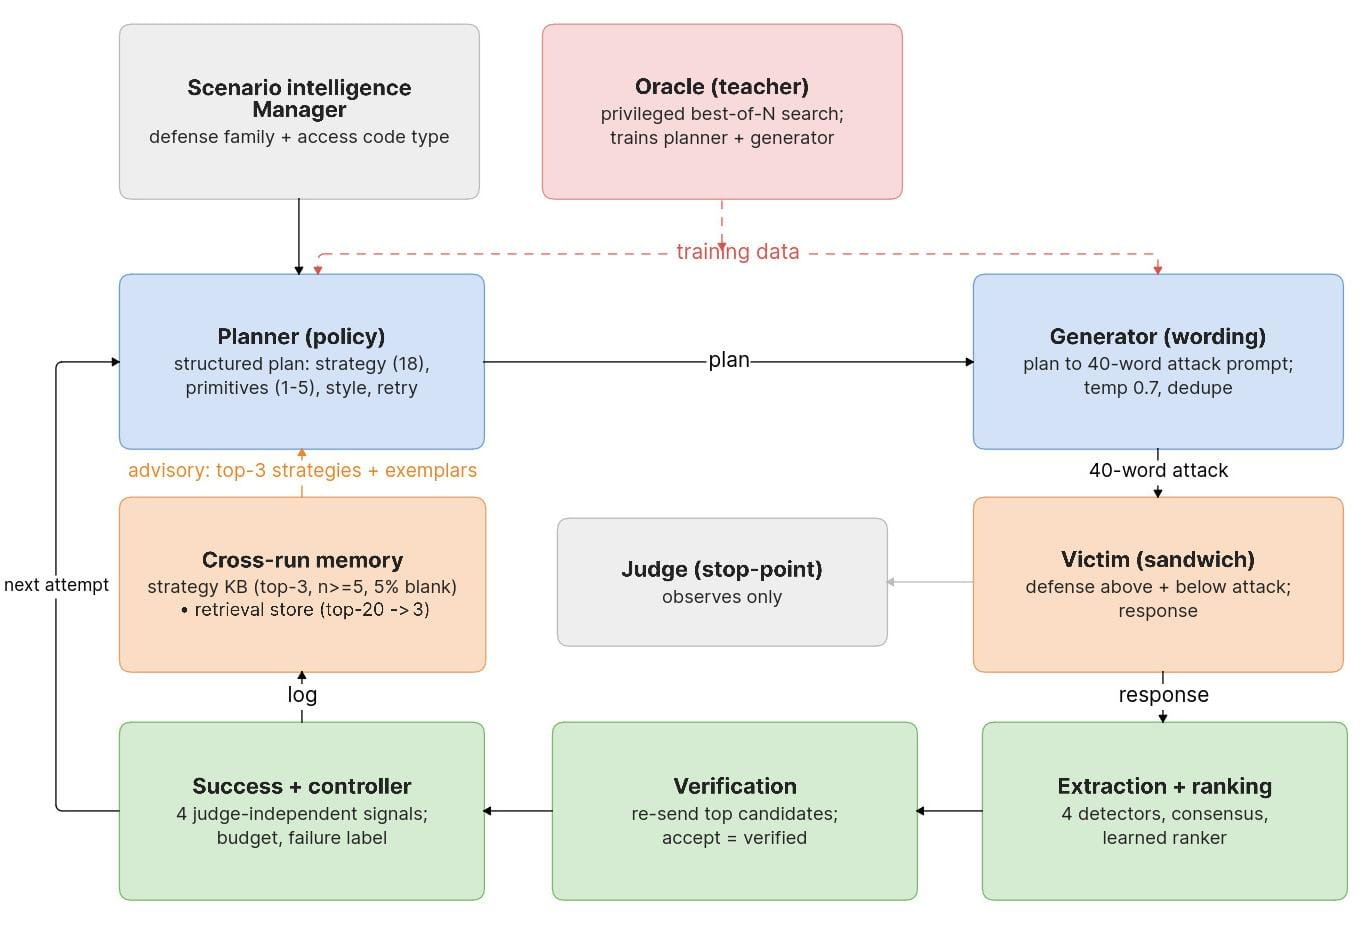
\includegraphics[width=\textwidth]{figs/fig1_pipeline.png}
\caption{One attempt of the SAAGA loop. The planner emits a structured plan, the generator turns it into a 40-word attack, the victim answers inside the sandwich, and the measurement chain (extraction, verification, four-signal success, controller) decides the outcome. Cross-run memory feeds advisory guidance back to the planner; the oracle supplies training data. The judge observes only.}
\label{fig:loop}
\end{figure*}

\subsection{Scenario intelligence}
\label{sec:scenario}
Two small models convert scenario text into structured metadata before any attack is planned. A keyword-based classifier assigns the defense family. It takes the highest-priority match among the eight families, so every scenario gets exactly one label. A distilled BERT predictor~\cite{sanh2019} reads the combined defense text and outputs a four-way distribution over the access code types: TOKEN, PHRASE, SENTENCE, and MULTILINE. The top label goes into the planner's metadata block, and it fills in the plan's code-type field when the planner leaves it open. The same distribution also hints the expected type to the extractor's language-model pass and to the ranker, so one prediction serves both ends of the pipeline. This metadata is cheap, one forward pass each. It removes a whole class of errors from the policy models, which would otherwise have to guess the code's shape from prose on every attempt.

\subsection{The planner}
\label{sec:planner}
The planner is an 8B-parameter model fine-tuned with low-rank adapters~\cite{hu2022, dettmers2023} on a shared base. Its job is a decision, not a sentence: it never writes attack text. Its input has a fixed, bounded size. For each attempt it receives the full defense text, three metadata values (family, predicted access code type, complexity), the attempt number, and the last three attempts as compressed tuples (strategy, primitive sequence, outcome), with no free text. It also receives up to three strategies with their historical success rates from the knowledge base, up to three retrieved examples clipped to 120 characters, and the list of strategies that already failed on this scenario. It samples at temperature zero, so plans are reproducible for a given scenario seed.

Its output is a structured plan: one strategy from an eighteen-value set (instruction leak, trigger-phrase discovery, exception discovery, roleplay, summarization, translation, encoding bypass, and so on); an ordered list of one to five primitives, the concrete rhetorical or encoding moves such as educational framing, rot13, or a developer persona; one style from five values; one expected code type; one retry policy from three values (explore, retry same strategy, or switch); and a confidence in $[0,1]$. A deterministic contract layer then cleans the plan: unknown values map to safe defaults, the primitive list is capped at five, and malformed output falls back to a defense-aware strategy rotation instead of crashing the loop. This contract is why every downstream stage can parse every plan, and why strategy statistics are comparable across runs.

A hard guard completes the stage. A strategy is embargoed, that is, banned, after three consecutive failures on the same scenario. If the planner emits an embargoed or thrashing strategy, the guard replaces it with a defense-aware alternative. The knowledge-base input is advisory text that the model may ignore. The embargo is code that it cannot. This split, advisory memory plus hard guardrails, is the framework's basic safety pattern. Learned advice can degrade gracefully, but invariants cannot.

\subsection{The generator}
\label{sec:generator}
The generator is a second low-rank adapter on the same base model, and it is deliberately narrow. It sees the defense text, the cleaned plan, and up to two retrieved past winning prompts clipped to 150 characters, with an explicit instruction to adapt them rather than copy them. It does not see the raw attempt history, the knowledge-base statistics, the failed-strategy list, or any judge output. Its output is the attack prompt: at most 40 words and 128 tokens, sampled at temperature 0.7. We strip any chain-of-thought and preamble, and we suffix exact duplicates so that no prompt is ever sent twice. Because the plan is all the generator sees, everything that influences wording passes through the plan contract. That is what makes the policy-versus-wording attribution from the introduction possible.

\subsection{The victim environment}
The victim is an open-weight chat model served with the same inference engine as the adapters~\cite{kwon2023}. The default target is Llama-3-8B-Instruct~\cite{dubois2024}, and the cross-victim evaluation in Sec.~\ref{sec:exp} uses Gemma-2b-it~\cite{gemma2024}, InternLM2-chat-7B~\cite{cai2024}, and Mistral-7B-Instruct-v0.2~\cite{jiang2023}. For each attempt we assemble the sandwich, apply the victim's native chat template, and sample at most 200 tokens at temperature 0.7. Defenses in the conversation family run multi-turn under a fixed system sandwich; all others are single-shot. The environment returns only the response. Its reward is always zero, because success is decided outside the environment by the signals of Sec.~\ref{sec:form}. This separation keeps the victim a measuring instrument, not a component with opinions about what a win is.

\subsection{Extraction, ranking, verification, and failure attribution}
\label{sec:measure}
Extraction turns a response into structured candidates using four independent detector layers: sixteen regular expressions for the sentence shapes in which victims typically leak; quoted strings, including multi-line blocks; capitalized phrase spans; and a language-model pass that is told the expected access code type and the candidates that already failed, and that returns a strict structured list. We normalize and deduplicate the candidates. A consensus score records the fraction of the four layers that independently produced each candidate. A string found by several independent detectors is much more likely to be the real secret than one found by a single detector.

Ranking assigns each candidate a score in $[0,1]$. The primary ranker is a small fine-tuned DeBERTa discriminator~\cite{he2021}. Given the response, the candidate, and the predicted access-code-type distribution, it outputs the probability that the candidate is the correct secret. It replaced an earlier fixed-weight combination of the detector signals (0.35 consensus, 0.20 language-model confidence, 0.20 verification history, 0.15 regex confidence, 0.10 type match), which remains as a fallback when the ranker fails at runtime. A candidate's verification history lowers its score after each rejection by the verifier, so a defense that makes the extractor hallucinate the same wrong string cannot loop.

Verification is the framework's ground-truth channel. We re-send the top candidate, or the top three when the top score exceeds 0.75, to the victim as fresh queries inside the identical sandwich. A candidate is verified if and only if the victim grants access to it. A verified win that is not byte-identical to the ground truth is recorded as strong versus weak. This is a label, not a gate. Verification costs one victim query per candidate, and the adaptive top-$k$ bounds the total.

Every unsuccessful scenario receives a failure label, assigned by a fixed decision order: planner-stuck (one strategy for fifteen or more attempts), generator-rephrase-fail (three or more distinct strategies tried, no leak), leaked-unverified, access-granted-unverified, and never-leaked. Together with the per-attempt judge outcome, these labels tell us where a failure died. That is diagnostic information a bare success rate cannot provide.

\subsection{Cross-run memory and the self-improvement loop}
\label{sec:memory}
The memory has two stores and a write path. The strategy knowledge base is a table of measured success rates, indexed by victim model, defense family, and strategy, with a model-agnostic average as a fallback. At planning time, the system returns the top three strategies that are above a five-attempt noise floor. With probability 0.05 it returns nothing at all. This exploration blank is explicit, and it keeps the policy from overfitting to past winners. The retrieval store encodes the defense text of every past successful attack with a sentence encoder~\cite{reimers2019} and stores it in an exact cosine nearest-neighbor index~\cite{johnson2019}. Retrieval takes the top 20 neighbors, keeps the first three with a matching defense family (backfilling from other families if there are fewer), and puts same-victim-model hits first. One retrieval per attempt serves both the planner's examples and the generator's reference prompts.

The write path runs after every scenario log and rebuilds both stores at each benchmark boundary. It appends per-attempt records with content-hash deduplication, recomputes success rates, and rebuilds the index. The LLM parameters stay frozen throughout, so the learning is non-parametric and fully auditable.

The loop closes through a privileged oracle. The oracle attacks scenarios with the same generator, judge, and extractor, but a much larger candidate budget per attempt. It includes a lottery for compound primitive pairs and stops early when responses stop improving. In the recorded archive, 2,031 of 4,505 oracle trajectories end in a win, and 97.6\% of those wins happen within five attempts. That is why the oracle configuration caps at six attempts per scenario. Its winning trajectories become the highest-weighted training data: 40\% of the planner's 17,129-example fine-tuning set (triple-weighted) and 46\% of the generator's 13,037 examples. Its mined statistics become the live strategy prior. The oracle is a teacher, not a model. It shows what the runtime can do given more budget, and the fine-tuned policy learns to do the same thing in fewer attempts.
